\documentclass[english,twoside, openright, hidelinks, 11 pt, class=report,crop=false]{standalone}
\input{../bm}
\input{../../preamb}


\begin{document}
\section{GeoGebra}
\subsection{Introduksjon}
Når du åpner GeoGebra får du et bilde som dette:
\begin{figure}[H]
	\centering
	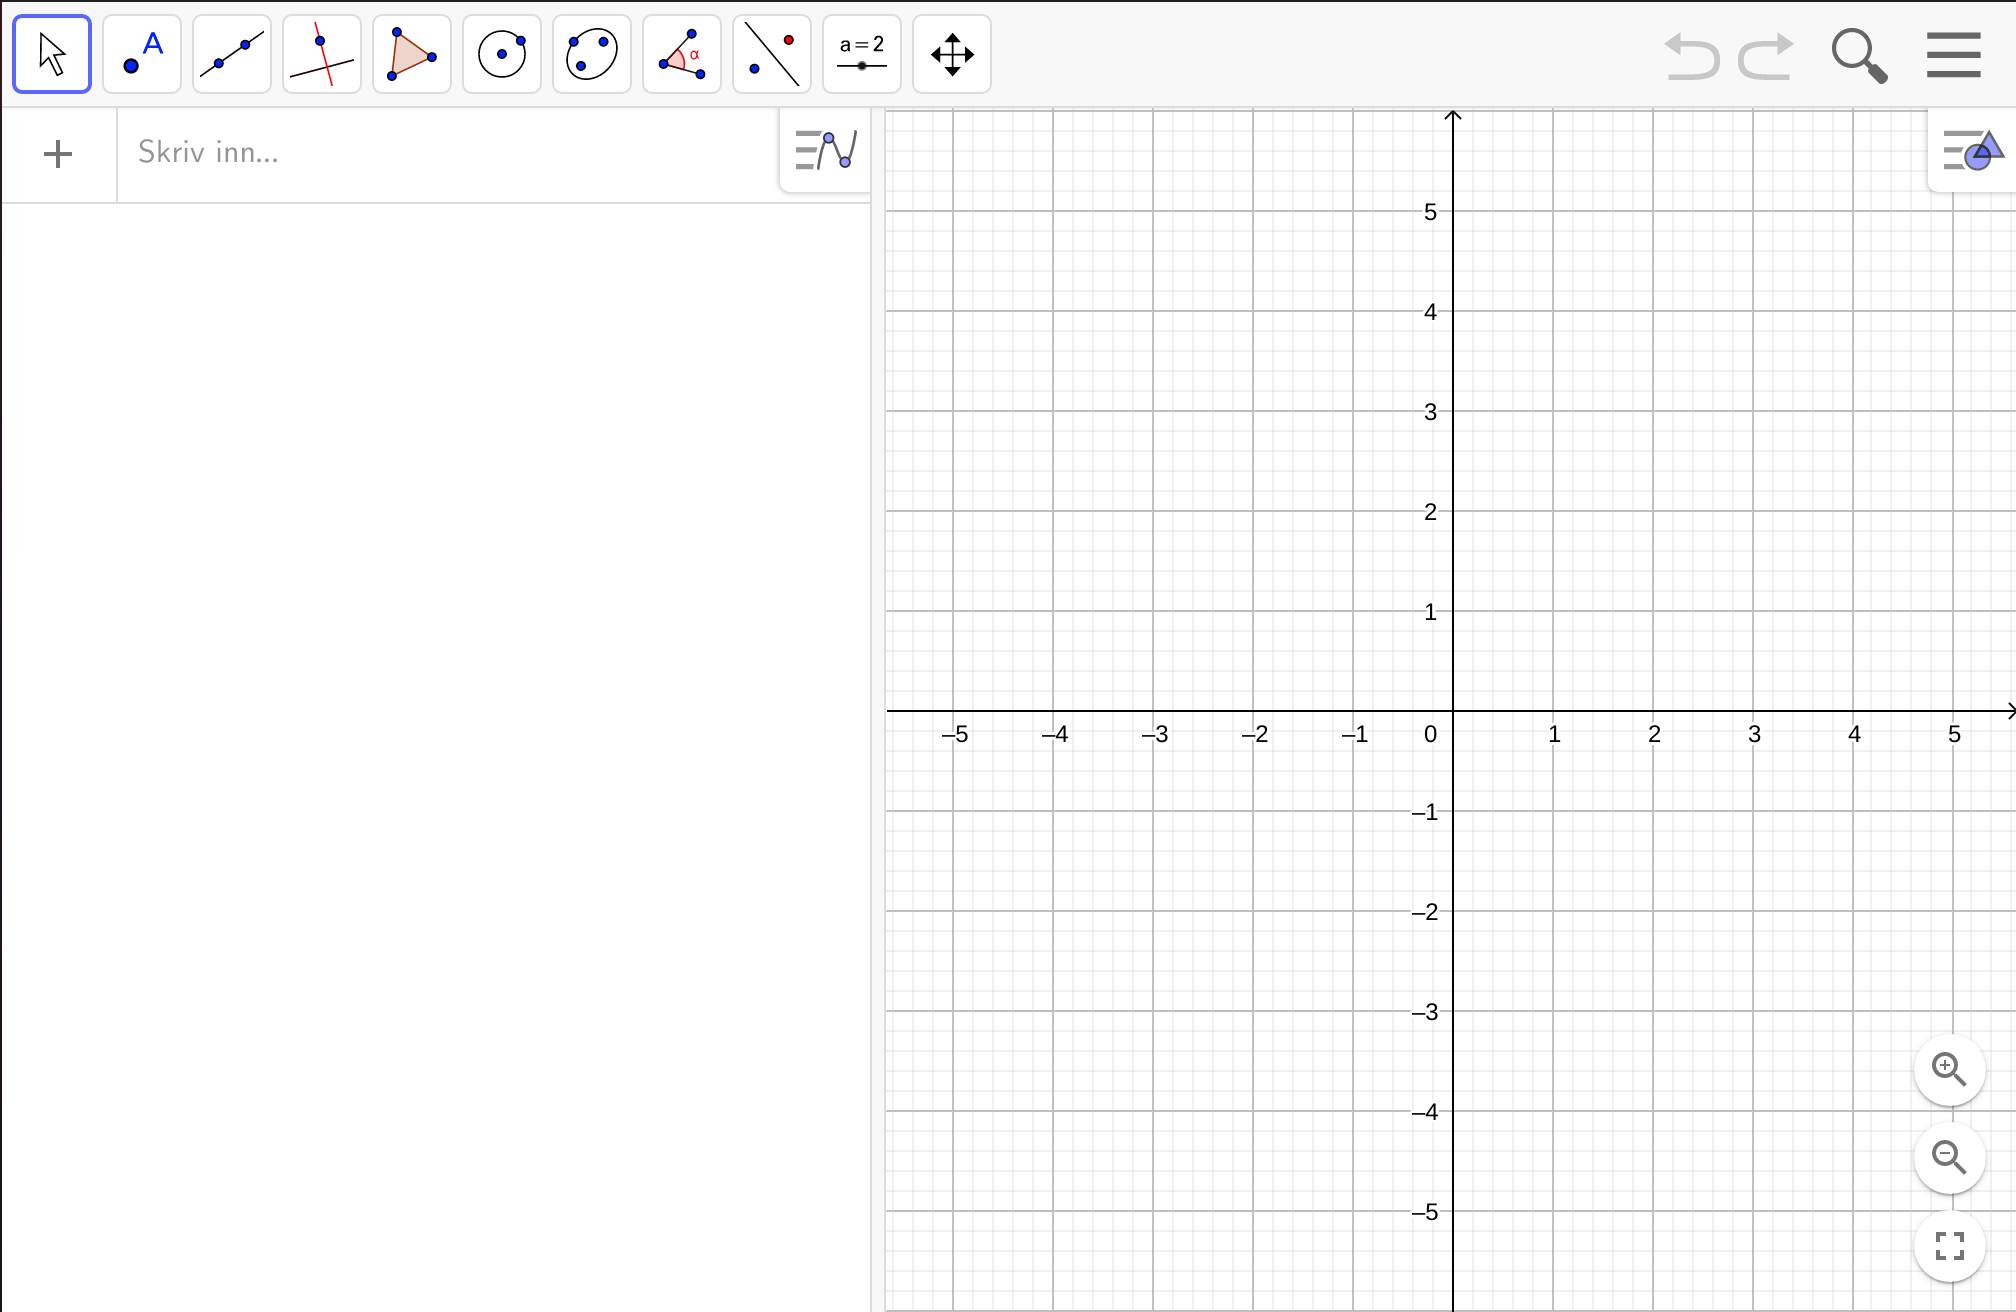
\includegraphics[scale=0.1]{ggbalgoggraf}
\end{figure}
Feltet hvor det står ''Skriv inn'' kalles \textit{inntastingsfeltet}. Dette feltet og det blanke feltet under utgjør \textit{algebrafeltet}. Koordinatsystemet til høyre kalles \textit{grafikkfeltet}.

\subsection{Å skrive inn punkt, funksjoner og linjer}
\subsubsection{Punkt}
Si at vi ønsker å få punktene $ (1,3) $ og $ (4,5) $ til å vises i grafikkfeltet. I inntastingsfeltet skriver vi da
\g{(1,3)}
og \vs
\g{(4,5)}
GeoGebra kaller da punktene $ A $ og $ B $, og tegner dem inn i grafikkfeltet:
\begin{figure}[H]
	\centering
	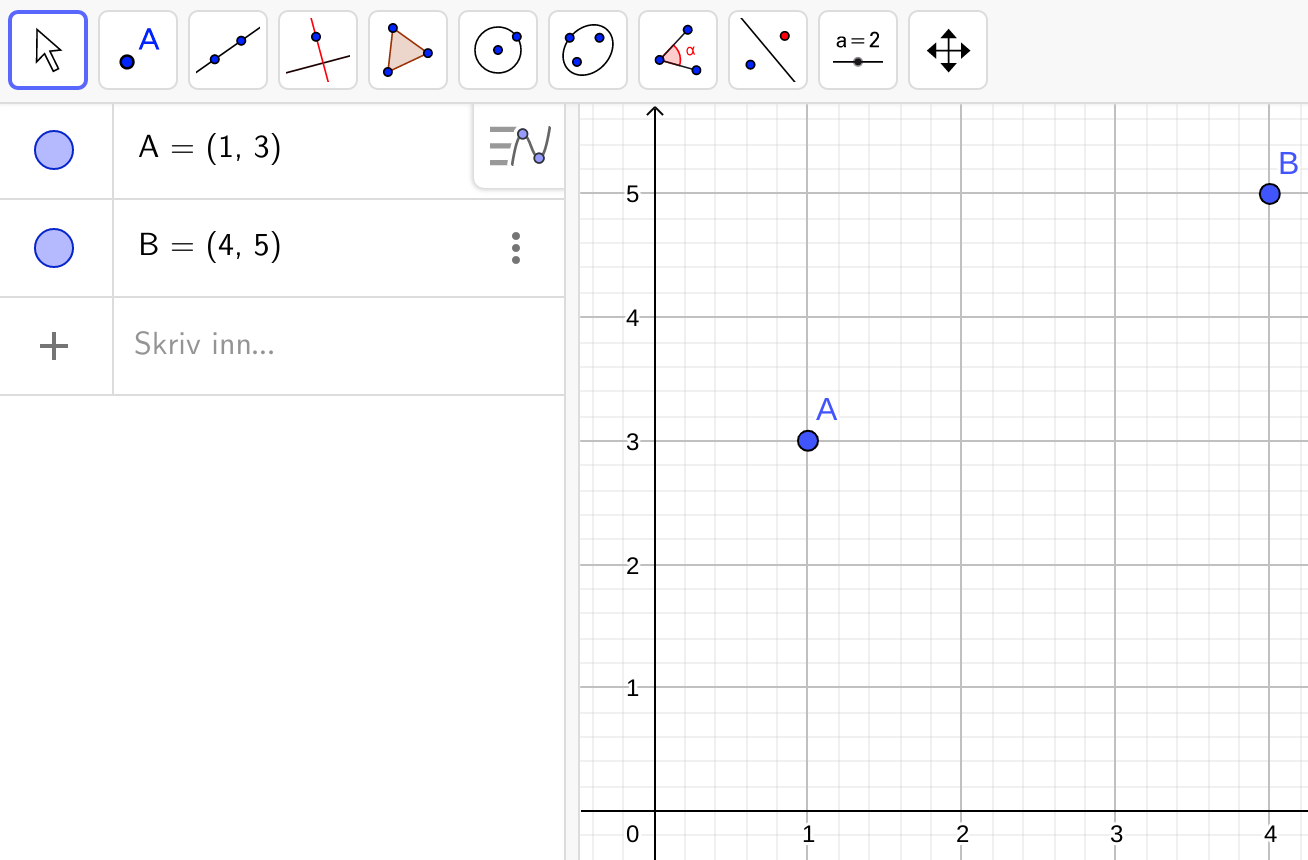
\includegraphics[scale=0.15]{pointAandB}
\end{figure}
Ønsker vi å bestemme et punkts navn kan vi f. eks skrive
\g{P=(2,4)}
\begin{figure}[H]
	\centering
	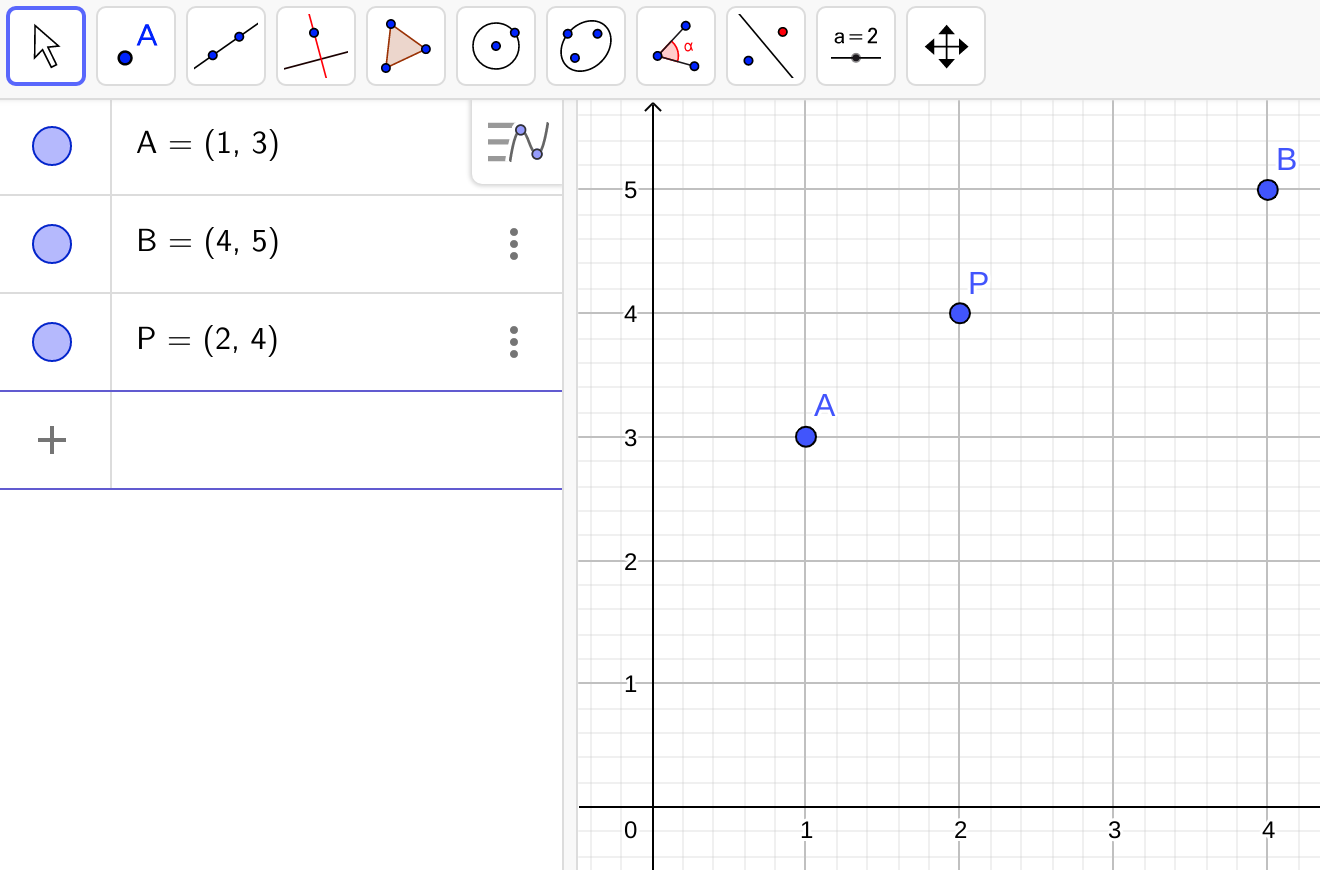
\includegraphics[scale=0.15]{pointP}
\end{figure}
\subsubsection{Funksjoner}
Si vi har funksjonen 
\[f(x)= \frac{3}{2} x^2 + 3x \]
For å bruke $ f(x) $ i GeoGebra, skriver vi:
\g{3/2*x\^{}2+3x}
Når vi ikke gir funksjonen noen navn, vil GeoGebra automatisk gi funksjonen navnet $ f $. I algebrafeltet får vi derfor
\begin{figure}[H]
	\centering
	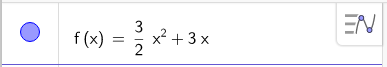
\includegraphics[scale=0.5]{skrivf}
\end{figure}
I grafikkfeltet får vi grafen til $ f $. \vsk

Hvis vi isteden har funksjonen
\[ P(x)= 0,15x^3 - 0,4 x\]
er det to ting vi må passe på. Det første er at \textsl{alle desimaltall må skrives med punktum istedenfor komma} i GeoGebra
. Det andre er at vi ønsker å gi funksjonen navnet $ P(x) $. Vi skriver da
\g{P(x) = 0.15x\^{}3 - 0.4x}
og får \vspace{-5pt}
\begin{figure}[H]
	\centering
	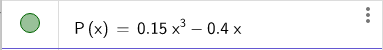
\includegraphics[scale=0.5]{pfig}
\end{figure}
\info{Obs!}{
Man kan aldri gi funksjoner navnet $ {y(x)} $ i GeoGebra. $ y $ kan bare brukes når man skriver inn uttrykk for en rett linje, altså $ {y=ax +b} $, hvor $ a $ og $ b $ er to valgfrie tall.
}

\subsubsection{Vannette og loddrette linjer}

Ønser vi å lage ei linje som går vannrett gjennom verdien 3 på $ y $-aksen og ei linje som går loddrett gjennom verdien 2 på $ x $-aksen skriver vi:
\g{y = 3}
og 
\g{x = 2 }
Da får vi denne figuren:
\begin{figure}[H]
	\centering
	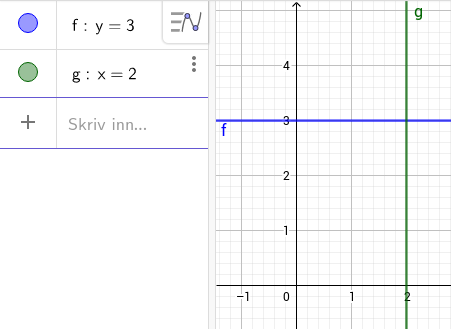
\includegraphics[scale=0.5]{23}
\end{figure}

\subsection{Å finne verdien til funksjoner og linjer}
\subsubsection{Funksjoner}
Si vi har funksjonen
\[H(x)= x^2 + 3x -3 \]
Hvis vi ønsker å vite hva $ H(2) $ er, skriver vi
\g{H(2)}
som resulterer i dette
\begin{figure}[H]
	\centering
	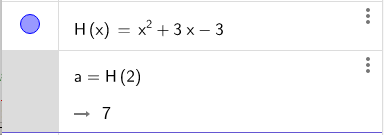
\includegraphics[scale=0.5]{H}
\end{figure}
Da vet vi at $ H(2)=7 $.
\subsubsection{Linjer}
Det anbefales på det sterkeste at du bruker funksjonsuttrykk når du behandler linjer i GeoGebra, men i noen tilfeller kommer man ikke utenom linjer på former $ y=ax+b $. \vsk

La oss se på de to linjene \vs
\alg{
	y&= x-3 \vn
	y&= -2x+1
}
Vi skriver disse inn i GeoGebra, og får
\begin{figure}[H]
	\centering
	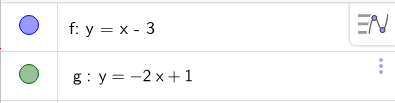
\includegraphics[scale=0.5]{fglin1}
\end{figure}
Ønsker vi nå å finne hva verdien til $ {y=x-3} $ er når $ {x=2} $, må vi legge merke til at GeoGebra har kalt denne linja for $ f $. Svaret vi søker får vi da ved å skrive $ f(2) $. Ønsker vi samtidig å vite hva $ {y=-2x+1} $ er når $ {x=0} $, må vi skrive $ g(0) $:
\begin{figure}[H]
	\centering
	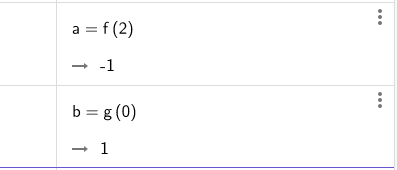
\includegraphics[scale=0.6]{fglin2}
\end{figure}
\newpage
\subsection{CAS}	
\subsubsection{Definere variabler \label{defvar}}
Hvis vi ønsker å definere variabler som vi skal bruke i andre celler, må vi skrive \texttt{:=} . I figuren under er forskjellen mellom \texttt{=} og \texttt{:=} demonstrert med et forsøk på å finne $ f'(x) $ til funksjonen $ f(x)=x^2 $:
\begin{figure}
	\centering
	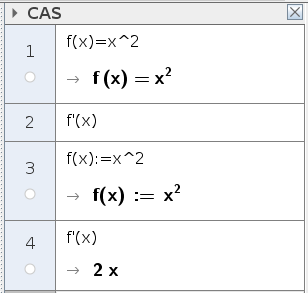
\includegraphics[scale=0.5]{fig/fder}
\end{figure}
Av figuren legger vi også merke til at celle 3 og celle 4 er markert med en hvit runding. Dette indikerer at størrelsen vil vises i \textsl{Grafikkfelt} eller \textsl{Grafikkfelt 3D} hvis man trykker på markøren (den skal da bli blå).
\subsubsection{Celle-referanser}

Ofte kommer vi ut for situasjoner der vi ønsker å bruke uttrykket vi har funnet i tidligere celler. Som eksempel har vi i celle 1 skrevet inn volumet $ v $ av en kule med radius $ r $, mens i celle 2 har vi volumet $ V $ av en kule med radius $ R $. Ønsker vi å finne forholdet mellom disse, kan vi bruke cellereferanser som hjelpemiddel. For å referere til celle 1 skriver vi \texttt{\$1} og for celle 2 skriver vi \texttt{\$2}. Forholdet $ \frac{v}{V} $ kan vi da skrive som \texttt{\$1/\$2}:
\begin{figure}
	\centering
	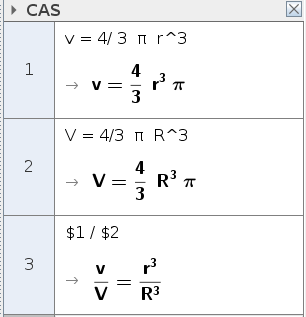
\includegraphics[scale=0.5]{fig/ref}
\end{figure}

\subsubsection{Lister}
Når et uttrykk står inni sløyfeparenteser \{\}, betyr det at det er laget en liste. En liste inneholder flere elementer som vi kan hente ut ved \texttt{Element}-kommandoen.
\begin{figure}
	\centering
	
\includegraphics[scale=0.5]{fig/liste}
\end{figure}
For å løse ligninger med flere ukjente kan vi bruke lister:
\begin{figure}
	\centering
	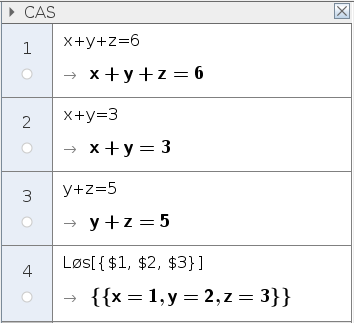
\includegraphics[scale=0.5]{fig/lign}
\end{figure}
\subsubsection{Høyre- og venstresiden \label{hogl}}
De fleste uttrykkene vi jobber med i CAS inneholder \texttt{=} er ligninger med en venstre- og høyreside. Ofte ønsker vi å bruke uttrykket på bare én av disse sidene, og oftest høyresiden. Som eksempel har vi løst ligningen $ (a+b)x = c $ og definert funksjonen $ f(x)= d x^2 $. Vi ønsker så å sette løsningen av ligningen inn i funksjonen. Dette gjør vi ved hjelp av \texttt{HøyreSide}-kommandoen:
\begin{figure}
	\centering
	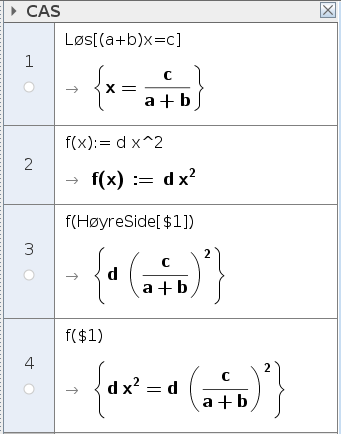
\includegraphics[scale=0.5]{fig/hoyre}
\end{figure}
\newpage
\subsubsection{ByttUt}
For å endre variabelen i et uttrykk, kan vi bruke \texttt{ByttUt}-kommandoen. La oss se på uttrykket
\[ \frac{a+b}{c} \]
Vi ønsker nå å sette $ {a=d }$, $ {b=2} $ og $ {c=f} $. Dette kan vi gjøre ved å skrive
\begin{figure}
	\centering
	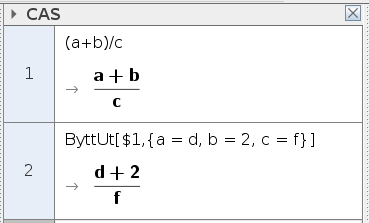
\includegraphics[scale=0.5]{fig/cas2}
\end{figure}	
\newpage
\subsection{Knapper og kommandoer}

\subsubsection*{Grafikkfelt}
Knappene velges fra rullemenyer på verktøylinjen. Nummereringen av menyene er fra venstre.\vsk

\begin{tabular}{@{}l}
	\,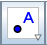
\includegraphics[scale=0.4]{fig/pkt} Lager et nytt punkt. (Meny nr. 1) \\
	\,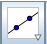
\includegraphics[scale=0.4]{fig/lin} Lager linje mellom to punkt. (Meny nr. 2)\\	
	\,
\includegraphics[scale=0.4]{fig/ekst} Finner topp- og bunnpunkt til en funksjon. (Meny nr. 2)\\
	\,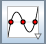
\includegraphics[scale=0.4]{fig/nul} Finner nullpunktene til en funksjon. (Meny nr. 2)	\\
	\,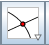
\includegraphics[scale=0.4]{fig/skj} Finner skjæringspunkt mellom to objekt. (Meny nr. 3)\\	
	\,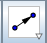
\includegraphics[scale=0.4]{fig/vek} Lager vektoren mellom to punkt (Meny nr. 3)\\		
	\,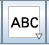
\includegraphics[scale=0.4]{fig/tekst} Lager en tekstboks. (Meny nr. 10)\\		
	\,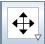
\includegraphics[scale=0.4]{fig/flytt} Flytter grafikkfeltet. Endrer verdiavstanden hvis man peker på aksene. \\
	\hspace{1cm}(Meny nr. 10)\\			
\end{tabular}
\subsubsection*{CAS}
\begin{tabular}{@{}l}
	\;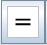
\includegraphics[scale=0.4]{fig/erlik} Gjengir uttrykket som er inntastet, ofte i forkortet form.\\	
	\;
\includegraphics[scale=0.4]{fig/brin} Gjengir uttrykket som er inntastet.\\	
	\;
\includegraphics[scale=0.4]{fig/caerlik} Gir tilnærmet verdi av et uttrykk (som desimaltall). \\	
	\;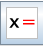
\includegraphics[scale=0.4]{fig/x} Gir eksaktløsningen av en ligning.\\
	\;
\includegraphics[scale=0.4]{fig/xca} Gir tilnærmet løsning av en ligning som desimaltall.\\
	
\end{tabular}
\subsubsection{Hurtigtaster}
\begin{tabular}{@{}c | c |c | c }
	&\textbf{Beskrivelse} & \textbf{PC }& \textbf{Mac} \\ \hline
	$ \sqrt{} $	& kvadratrot& \texttt{alt\,+\,r} &\texttt{alt\,+\,r} \\\hline
	$ \pi $	& pi& \texttt{alt\,+\,p} & \texttt{alt\,+\,p}\\\hline
	$ \infty $ &uendelig& \texttt{alt\,+\,u} &\texttt{alt\,+\,,}  \\\hline
	$ \otimes $&kryssprodukt & \texttt{alt\,+\,shift\,+\,8}&\texttt{ctrl\,+\,shift\,+\,8} \\\hline
	$ e $&eulers tall & \texttt{alt\,+\,e}& \texttt{alt\,+\,e}\\\hline
	$ {}^\circ $&gradtegnet ($ \frac{\pi}{180} $) & \texttt{alt\,+\,o}& \texttt{alt\,+\,o}
	\\\hline	
\end{tabular}

\newpage
\subsubsection{Kommandoliste for grunnskole og P-fag}
\mers{Mange av kommandoene har egne knapper, som blant annet vist i videoene i neste avsnitt.}
\begin{itemize}
	\item \cmds{abs( <x> )}{Gir lengden til $ x $ (et tall, et linjestykke o.l.). Alternativt kan man skrive {\tt{|x|}}}.
	
	\item \cmds{Avstand( <Punkt>, <Objekt> )}
	{Gir avstanden fra et punkt til et objekt.}
	
	\item \cmds{Linje( <Punkt>, <Punkt> )}{Gir linjen mellom to punkt.}
	
	\item \cmds{Ekstremalpunkt( <Funksjon>, <Start>, <Slutt> )}{Finner lokale topp- og bunnpunkt til en funksjon på et gitt intervall.}
	
	\item \cmds{Ekstremalpunkt( <Polynom> )}
	{Finner lokale topp- og bunnpunkt til et polynom.}
	
	\item \cmds{Funksjon( <Funksjon>, <Start>, <Slutt> )}{Tegner en funksjon innenfor et gitt intervall.}
	
	\item \cmds{Mangekant( <Punkt>, ..., <Punkt> )}{Tegner mangekanten mellom gitte punkt.}
	
	\item \cmds{Løs ( <Likning med x> )}{
		Løser en likning med $ x $ som ukjent.
	}
	
	\item 
	\cmds{Løs( <Liste med likninger>, <Liste med variabler> )}
	{Finner alle løsninger av en liste med ligninger med gitte variabel som ukjente.}
	
	\item \cmds{Løs( <Likning>, <Variabel> )}
	{Finner alle løsninger av en gitt likning med en gitt variabel som ukjent.}
	
	\item \cmds{Nullpunkt( <Funksjon>, <Start>, <Slutt> )}{Gir nullpunktene til en funksjon innenfor et gitt intervall}
	
	\item \cmds{RegLin( <Liste> )}
	{Bruker regresjon med en rett linje for å tilpasse punkt gitt i en liste.}
	
	\item \cmds{RegEksp( <Liste> )}
	{Bruker regresjon med en eksponentialfunksjon for å tilpasse punkt gitt i en liste.}
	
	\item \cmds{RegPoly( <Liste>, <Grad> )}
	{Bruker regresjon med et polynom av gitt grad for å tilpasse punkt gitt i en liste.}
	
	\item \cmds{RegPot( <Liste> )}
	{Bruker regresjon med en potensfunksjon for å tilpasse punkt gitt i en liste.}
	
	\item \cmds{Skjæring( <Objekt>, <Objekt> )}{Finner skjæringspunktene til to objekt (funksjoner, linjer o.l.)}
	
	\item \cmds{Vinkel( <Punkt>, <Toppunkt>, <Punkt> )}{
	Finner verdien til vinkelen dannet av tre punkt.
	}
\end{itemize}

\subsubsection{Kommandoliste for 1T, R1 og R2}
\mers{Denne listen er en fortsettelse av den forrige kommandolisten. Tar du fagene 1T, R1 eller R2 bør du kjenne til kommandoene fra begge listene.}
\begin{itemize}
	
	\item \cmds{acos( <x> )}
	{
		I algebrafelt: Gir vinkelen på intervallet $ [0^\circ, 180^\circ] $ som har cosinus-verdi $ x $. \os
		I CAS: Gir vinkelen på intervallet $ [0, \pi] $ som har cosinus-verdi $ x $.
	}
	
	\item \cmds{acosd( <x> )}
	{
		I algebrafelt: Gir vinkelen på intervallet $ [0^\circ, 180^\circ] $ som har cosinus-verdi $ x $.
	}
	
	\item \cmds{asin( <x> )}
	{
		I algebrafelt: Gir vinkelen på intervallet $ [-90^\circ, 90^\circ] $ som har sinus-verdi $ x $.\os
		
		I CAS: Gir vinkelen på intervallet $ [-\frac{\pi}{2}, \frac{\pi}{2}] $ som har sinus-verdi $ x $.
	}
	
	\item \cmds{asind( <x> )}
	{
		Gir vinkelen på intervallet $ [-90^\circ, 90^\circ] $ som har sinus-verdi $ x $.
	}
	
	\item \cmds{atan( <x> )}
	{
		I algebrafelt: Gir vinkelen på intervallet $ [-90^\circ, 90^\circ] $ som har tangens-verdi $ x $.\os
		
		I CAS: Gir vinkelen på intervallet $ [-\frac{\pi}{2}, \frac{\pi}{2}] $ som har tangens-verdi $ x $.
	}
	
	\item \cmds{atand( <x> )}
	{
		Gir vinkelen på intervallet $ [-90^\circ, 90^\circ] $ som har tangens-verdi $ x $.
	}
	
	
	\item \cmds{Asymptote( <Funksjon> )}
	{Finner asymptotene til en funksjon.}
	
	
	

	
	\item \cmds{ByttUt( <Uttrykk>, <Liste med forandringer> ) }
	{Viser et gitt uttrykk etter endring av variabler, gitt i en liste.}
	
	\item \cmds{Deriverte( <Funksjon> )}{Gir den deriverte av en funksjon.\\	
		\mers{
			For en definert funksjon $ f(x) $, kan man like gjerne skrive \texttt{f'(x)}.
	}}
	
	\item \cmds{Divisjon ( <Dividend Polynom >, <Divisor Polynom> )}{
		Gir kvotienten og resten til en polynomdivisjon.
	}
	

	
	\item \cmds{Element( <Liste>, <Posisjonen til elementet> )}
	{
		Gir elementet til en liste ut ifra en gitt posisjon.
	}
	
	\item \cmds{Faktoriser ( <Tall/Polynom> )}{
		Faktoriserer et tall/polynom.
	}
	

	\item \cmds{Høyde( <Objekt> )}
	{Gir avstanden fra toppunkt til grunnflate i et objekt.\\ 
		\mers{Avstanden har retning, og derfor kan den noen ganger være negativ. Tallverdien er den geometriske høyden.}}
	
	\item \cmds{HøyreSide ( <Likning> )}
	{Gir høyresiden til en likning.}
	
	\item \cmds{HøyreSide ( <Liste med likninger> )}
	{Gir en liste med høyresidene i en liste med ligninger.}
	
	\item \cmds{Integral ( <Funksjon> )}
	{Gir uttrykket til det ubestemte integralet av en funksjon. \\
		\mers{Hvis kommandoen skrives i inntastingsfeltet, blir konstantleddet utelatt}
	}
	
	\item \cmds{Integral( <Funksjon>, <Start>, <Slutt> )}
	{Gir det bestemte integralet av en funksjon på et intervall.}
	
	\item \cmds{Integral( <Variabel> )}
	{Gir uttrykket til det ubestemte integralet til en funksjon av gitt variabel. (Brukes dersom man ønsker å integrere funksjoner avhengig av en annen variabel enn $ x $).}
	
	\item \cmds{Kule( <Punkt>, <Radius> )}
	{Viser en kule i Grafikkfelt 3D med sentrum i et gitt punkt og med en gitt radius.}
	
	\item \cmds{Kurve( <Uttrykk>, <Uttrykk>, <Uttrykk>, <Parametervariabel>, <Start>, <Slutt> )}
	{Viser parameteriseringen av en kurve i Grafikkfelt 3D på et gitt intervall. Uttrykkene er henholdsvis uttrykkene for $ {x, y} $ og $ z $-koordinatene, bestemt av en gitt parametervariabel. \\
		\mers{
			Med mindre et bestemt intervall av kurven er ønsket, er det bedre å skrive parameteriseringen direkte inn i inntastingsfeltet som \texttt{A+t*u}, hvor $ A $ er et punkt på linja og $ u$ er en retningsvektor.
	}}	
	
	\item \cmds{Linje ( <Punkt>, <Punkt> )}{ Gir uttrykket til en linje mellom to punkt. Hvis punktene har tre koordinater består uttrykket av et punkt på linja og en fri variabel $ \lambda $ multiplisert med en retningsvektor.}	
	
	\item \cmds{Maks( <Funksjon>, <Start x-verdi>, <Slutt x-verdi> )}{Finner absolutt maksimum og maksimalpunkt for en funksjon $ f $ på et gitt intervall.}
	
	\item \cmds{Min}( <Funksjon>, <Start x-verdi>, <Slutt x-verdi> ) {Finner absolutt minimum og minimumspunkt for en funksjon $ f $ på et gitt intervall.}
	
	\item \cmds{Nullpunkt( <Polynom> )}
	{Finner alle nullpunkter til et polynom.}
	
	\item \cmds{NullpunktIntervall( <Funksjon>, <Start>, <Slutt> )}
	{Finner alle nullpunkter på et gitt intervall til en hvilken som helst funksjon.}
	
	\item \cmds{Plan( <Punkt>, <Punkt>, <Punkt> )}
	{Viser et plan i Grafikkfelt 3D, utspent av to av vektorene mellom tre gitte punkt.}
	
	\item \cmds{Prisme( <Punkt>, <Punkt>, ... )}
	{Framstiller et prisme i Grafikkfelt 3D. {\tt Prisme[A,B,C,D]} lager et prisme med grunnflate $ ABC $ og tak $ DEF $, {\tt Prisme[A,B,C,D,E]} har grunnflate $ ABCD $ og tak $ EFG $. $ E, F$ og eventuelt $ G $ blir konstruert av GeoGebra slik at hver sideflate er et parallellogram. Under kategorien \textsl{Prisme} i algebrafeltet finner man en konstant som oppgir volumet til prismen.}
	
	\item \cmds{Pyramide( <Punkt>, <Punkt>, ... )}
	{Framstiller en pyramide i Grafikkfelt 3D. {\tt Pyramide[A,B,C,D]} lager en pyramide med grunnflate ${ A, B, C} $ og toppunkt $ D $, mens {\tt Pyramide[A,B,C,D, E]} har grunnflate ${ A, B, C, D }$ og toppunkt $ E $. Under kategorien \textsl{Pyramide} i algebrafeltet finner man en konstant som oppgir volumet til pyramiden.}
	
	\item \cmds{RegLogist( <Liste> )}
	{Bruker regresjon med en logistisk funksjon for å tilpasse punkt gitt i en liste.}
	
	\item \cmds{RegSin( <Liste> )}
	{Bruker regresjon med en sinusfunksjon for å tilpasse punkt gitt i en liste.}
	
	\item \cmds{Skalarprodukt( <Vektor>, <Vektor> )} 
	{Finner skalarproduktet av to vektorer. \\
		\mers{For to vektorer $u$ og $v$ kan man like gjerne skrive \texttt{u*v}.}}
	
	\item \cmds{Skjæring( <Objekt>, <Objekt> )}
	{Finner skjæringspunktene mellom to objekter. 
	}
	
	\item \cmds{Skjæring( <Funksjon>, <Funksjon>, <Start>, <Slutt> )}
	{Finner skjæringspunktene mellom to funksjoner på et gitt intervall.}
	
	\item \cmds{Sum( <Uttrykk>, <Variabel>, <Start>, <Slutt> )}{
		Finner summen av en rekke med en løpende variabel på et intervall.
	}
	
	\item \cmds{TrigKombiner( <Funksjon> )}
	{Skriver om et uttrykk på formen $ a\sin (kx) + b\cos (kx) $ til et kombinert uttrykk på formen $ r\cos (kx-c) $.}
	
	\item \cmds{TrigKombiner( <Funksjon>, sin(x) )}{Skriver om en funksjon på formen $ {a\sin (kx) + b\cos (kx) }$ til et kombinert uttrykk på formen $ r\sin (kx+c) $.}
	
	\item \cmds{Vektor( <Punkt> )}{
		Lager vektoren fra origo til et gitt punkt. \\
		\mers{I CAS kan man lage vektoren $ {[x, y]} $ ved å skrive \texttt{(x,y)}, dette anbefales.}
	}
	
	\item \cmds{Vektorprodukt( <Vektor>, <Vektor> )}{Finner vektorproduktet av to vektorer. \\
		\mers{For to vektorer $u$ og $v$ kan man like gjerne skrive \texttt{u}$ \otimes $\texttt{v}. }
	}
	
	\item \cmds{Vendepunkt( <Polynom> )}
	{Finner vendepunktene til et polynom.}
	
	\item \cmds{VenstreSide( <Likning> )}
	{Gir venstresiden til en likning.}
	
	\item \cmds{VenstreSide( <Liste med likninger> )}
	{Gir en liste med venstresidene i en liste med ligninger.}
	
	\item \cmds{Vinkel( <Vektor>, <Vektor> )}
	{Gir vinkelen mellom to vektorer. Kan også brukes for vinkel mellom plan/linjer, plan/plan og linje/linje}
	
	\item \cmds{X( <Punkt> )}{
		Gir $ x $-koordinaten til et punkt.
	}
	
	\item \cmds{Y( <Punkt> )}{
		Gir $ y $-koordinaten til et punkt.
	}
	
	\item \cmds{Z( <Punkt> )}{
		Gir $ z $-koordinaten til et punkt.
	}
\end{itemize}
\label{commandlistend}

\newpage
\subsection{Videoer}
\begin{itemize}
	\item \net{https://drive.google.com/file/d/1u9u6eZFW8yqtM2ukdW9716i1_YH0NMOa/view?usp=sharing}{Finne nullpunktene til en graf}
	\item \net{https://drive.google.com/file/d/11B7o3WMrbR5cpfshkv9FSBpQ5khBCwLS/view?usp=sharing}{Finne lokale bunnpunkt (eller toppunkt) til en graf}
	\item \net{https://drive.google.com/file/d/1koy-ffEejtIt-YbIohoFN4gbMLi-95cb/view?usp=sharing}{Finne skjæringspunktene til to funksjoner}
	\item \net{https://drive.google.com/file/d/1Z8v05XjlqsSFpHEed5q4s0nGDjdQUfqs/view?usp=sharing}{Justere akser}
	\item \net{https://drive.google.com/file/d/1oKKDk084IEhy11rNhDk0-VykzXLuhthy/view?usp=sharing}{Endre tykkelse, farge o.l på graf}
	\item \net{https://drive.google.com/file/d/1568rRj2PxzwK6wSm7v4w3GWzDnGtSuuX/view?usp=sharing}{Tegne graf på gitt intervall}	\\
	{\footnotesize I videoen tegner vi $f(x)= x^2-3x+2 $ på intervallet $ 0\leq x \leq 5 $}.
	\item \net{https://drive.google.com/file/d/1x7y7DJMJ-7rfpgapB48e5Nlq6UnXXcI2/view?usp=sharing}{Lage linje mellom to punkt}	\\
	{\footnotesize Legg merke til hva som gjøres mot slutten av videoen for å få det vante uttrykket $ y=ax+b $}.
	\item \net{https://drive.google.com/file/d/18cNeX3vJFEY7BpgrH_BFpI1q4c-bczyH/view?usp=sharing}{Utføre regresjon i algebrafelt}\\
	{\footnotesize I videoen har vi på forhånd skrevet inn tallene i tabellen under, som viser elbilsalget i Norge antall år etter 2010. Disse tallene ble også brukt i \refsec{Regresjon}. \os
		Det utføres regresjon med en linje, en kvadratisk funksjon og en 4. grads funksjon.
		
		\begin{tabular}{c|c}
			\textbf{antall år} & \textbf{elbiler} \\ \hline
			0 &	3347\\
			1 &	5381\\
			2 &	9565\\
			3 &	19678\\
			4 &	42356\\
			5 &	73312\\
			6 &	101126\\
			7 &	138477\\
			8 &	194900\\
			9 &	260688\\
			10 &337201\\
			11 &	455271\\
		\end{tabular}
	}
	\item \net{https://drive.google.com/file/d/1GYSaDyHt064yqmCBpfmbJATRDs6aWuBP/view?usp=sharing}{Regresjonsanalyse i regnearket}\\
	{\footnotesize I videoen finner vi hvilket polynom som best beskriver summen av de $ n $ første kvadrattallene ($ 1^2 $, $ 2^2 $, $ 3^2 $ og så videre). $ R^2 $ er et tall mellom 0 og 1 som viser hvor nærme funksjonen er å skjære gjennom hvert punkt, hvor $ R^2=1 $ betyr at funksjonen skjærer hvert punkt eksakt. 
		\begin{center}
			\begin{tabular}{c|c}
				\boldmath $ n $ & \textbf{sum}\\
				1 & 1\\
				2 & 5\\
				3 & 14 \\
				4 & 30 \\
				5 & 55	
			\end{tabular}
		\end{center}
	}
\end{itemize}


\end{document}

